\trilingualchapter{Financial Management: The Numbers Behind Success}{财务管理:成功背后的数字}{Finanzmanagement: Die Zahlen hinter dem Erfolg}{}

Financial management is the foundation of a sustainable restaurant business. While Sue brought culinary excellence and Owen brought operational expertise, both needed to master the financial aspects to ensure their restaurant's long-term success. This chapter covers budgeting, cost control, pricing, financial reporting, and profitability management.

\section{Understanding Restaurant Finances | 理解餐厅财务 | Restaurantfinanzen verstehen}

Restaurant financial management is unique due to:
\begin{itemize}
    \item High fixed costs (rent, labor, utilities)
    \item Variable costs tied to sales (food, beverages)
    \item Cash flow challenges (daily receipts, weekly payables)
    \item Thin profit margins (typically 3-5\%)
    \item Seasonality and fluctuations
\end{itemize}

\section{Key Financial Metrics | 关键财务指标 | Wichtige Finanzkennzahlen}

\begin{figure}[h]
\centering
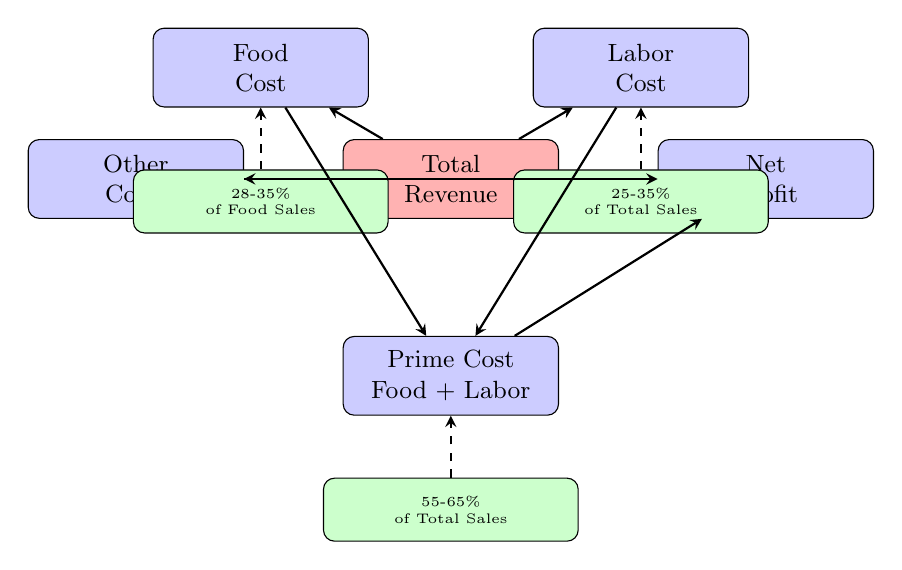
\begin{tikzpicture}[
    node distance=2cm,
    auto,
    metric/.style={rectangle, draw, fill=blue!20, text width=2.5cm, text centered, rounded corners, minimum height=1cm, font=\small},
    formula/.style={rectangle, draw, fill=green!20, text width=3cm, text centered, rounded corners, minimum height=0.8cm, font=\tiny},
    arrow/.style={thick,->,>=stealth}
]
    % Central revenue
    \node [metric, fill=red!30] (revenue) {Total\\Revenue};
    
    % Cost metrics
    \node [metric, above left of=revenue, xshift=-1cm] (food) {Food\\Cost};
    \node [metric, above right of=revenue, xshift=1cm] (labor) {Labor\\Cost};
    \node [metric, below of=revenue, yshift=-0.5cm] (prime) {Prime Cost\\Food + Labor};
    
    % Other costs
    \node [metric, left of=revenue, xshift=-2cm] (other) {Other\\Costs};
    \node [metric, right of=revenue, xshift=2cm] (profit) {Net\\Profit};
    
    % Formulas
    \node [formula, below of=food, yshift=0.3cm] (f1) {28-35\%\\of Food Sales};
    \node [formula, below of=labor, yshift=0.3cm] (f2) {25-35\%\\of Total Sales};
    \node [formula, below of=prime, yshift=0.3cm] (f3) {55-65\%\\of Total Sales};
    
    % Arrows
    \draw [arrow] (revenue) -- (food);
    \draw [arrow] (revenue) -- (labor);
    \draw [arrow] (food) -- (prime);
    \draw [arrow] (labor) -- (prime);
    \draw [arrow] (revenue) -- (other);
    \draw [arrow] (prime) -- (profit);
    \draw [arrow] (other) -- (profit);
    
    % Formula connections
    \draw [arrow, dashed] (f1) -- (food);
    \draw [arrow, dashed] (f2) -- (labor);
    \draw [arrow, dashed] (f3) -- (prime);
\end{tikzpicture}
\caption{Key Financial Metrics Relationships}
\label{fig:financial_metrics}
\end{figure}

\subsection{Primary Metrics}

\subsubsection{Food Cost Percentage}
\begin{equation}
\text{Food Cost \%} = \frac{\text{Cost of Food Sold}}{\text{Food Sales}} \times 100
\end{equation}
Target: 28-35\% of food sales

\subsubsection{Labor Cost Percentage}
\begin{equation}
\text{Labor Cost \%} = \frac{\text{Total Labor Costs}}{\text{Total Sales}} \times 100
\end{equation}
Target: 25-35\% of total sales

\subsubsection{Prime Cost}
\begin{equation}
\text{Prime Cost} = \text{Food Cost} + \text{Labor Cost}
\end{equation}
Target: 55-65\% of total sales

\subsubsection{Controllable Costs}
\begin{itemize}
    \item Food and beverage costs
    \item Labor costs
    \item Supplies and smallwares
    \item Marketing
    \item Repairs and maintenance
\end{itemize}

\subsubsection{Fixed Costs}
\begin{itemize}
    \item Rent
    \item Insurance
    \item Utilities (base charges)
    \item Loan payments
    \item Depreciation
\end{itemize}

\section{Budgeting and Forecasting | 预算与预测 | Budgetierung und Prognose}

\subsection{Annual Budget | 年度预算 | Jahresbudget}

Sue and Owen created an annual budget as their financial roadmap:

\subsubsection{Revenue Budget}
\begin{itemize}
    \item Monthly sales projections
    \item Based on:
    \begin{itemize}
        \item Seating capacity
        \item Average check size
        \item Table turnover
        \item Days open
        \item Seasonal patterns
        \item Growth trajectory
    \end{itemize}
\end{itemize}

\subsubsection{Expense Budget}
\begin{itemize}
    \item \textbf{Food costs}: Based on sales and target food cost \%
    \item \textbf{Beverage costs}: Based on sales and target beverage cost \%
    \item \textbf{Labor costs}: Based on sales and target labor cost \%
    \item \textbf{Occupancy costs}: Rent, CAM, utilities
    \item \textbf{Operating expenses}: Supplies, marketing, repairs
    \item \textbf{Fixed costs}: Insurance, loan payments, etc.
\end{itemize}

\subsection{Monthly Forecasting | 月度预测 | Monatliche Prognose}

\begin{itemize}
    \item Update projections based on trends
    \item Adjust for seasonality
    \item Account for special events
    \item Revise as needed
\end{itemize}

\section{Cost Control | 成本控制 | Kostenkontrolle}

\subsection{Food Cost Control | 食品成本控制 | Lebensmittelkostenkontrolle}

\subsubsection{Purchasing}
\begin{itemize}
    \item Negotiate best prices
    \item Buy in appropriate quantities
    \item Minimize waste
    \item Use seasonal ingredients
    \item Build supplier relationships
\end{itemize}

\subsubsection{Receiving}
\begin{itemize}
    \item Verify quantities and quality
    \item Check pricing
    \item Reject substandard items
    \item Proper storage immediately
\end{itemize}

\subsubsection{Storage}
\begin{itemize}
    \item Proper temperature control
    \item FIFO rotation
    \item Security (prevent theft)
    \item Regular inventory
\end{itemize}

\subsubsection{Preparation}
\begin{itemize}
    \item Standardized recipes
    \item Portion control
    \item Minimize waste
    \item Use all parts of ingredients
\end{itemize}

\subsection{Labor Cost Control | 人工成本控制 | Arbeitskostenkontrolle}

\subsubsection{Scheduling}
\begin{itemize}
    \item Forecast sales accurately
    \item Schedule based on business levels
    \item Avoid overstaffing
    \item Cross-train for flexibility
    \item Monitor daily labor costs
\end{itemize}

\subsubsection{Productivity}
\begin{itemize}
    \item Efficient workflows
    \item Proper training
    \item Clear expectations
    \item Performance management
    \item Technology utilization
\end{itemize}

\subsection{Other Cost Controls | 其他成本控制 | Weitere Kostenkontrollen}

\begin{itemize}
    \item \textbf{Utilities}: Energy-efficient equipment, monitoring
    \item \textbf{Supplies}: Bulk purchasing, inventory control
    \item \textbf{Marketing}: Track ROI, focus on effective channels
    \item \textbf{Repairs}: Preventive maintenance, vendor relationships
\end{itemize}

\section{Pricing Strategy | 定价策略 | Preisstrategie}

\subsection{Pricing Methods | 定价方法 | Preisgestaltungsmethoden}

\subsubsection{Cost-Plus Pricing}
\begin{equation}
\text{Selling Price} = \frac{\text{Food Cost}}{\text{Target Food Cost \%}}
\end{equation}
Example: If food cost is \$8 and target is 30\%, selling price = \$8 / 0.30 = \$26.67

\subsubsection{Competitive Pricing}
\begin{itemize}
    \item Research competitor prices
    \item Position relative to market
    \item Consider value proposition
\end{itemize}

\subsubsection{Value-Based Pricing}
\begin{itemize}
    \item Price based on perceived value
    \item Consider unique offerings
    \item Account for experience, not just food
\end{itemize}

\subsection{Pricing Considerations | 定价考虑 | Preisüberlegungen}

\begin{itemize}
    \item Target food cost percentage
    \item Labor costs
    \item Overhead allocation
    \item Competitive positioning
    \item Customer price sensitivity
    \item Profit margin goals
    \item Psychological pricing (\$19.95 vs \$20.00)
\end{itemize}

\section{Financial Reporting | 财务报告 | Finanzberichterstattung}

\subsection{Daily Reports | 日报 | Tagesberichte}

\begin{itemize}
    \item \textbf{Sales}: Total revenue, covers, average check
    \item \textbf{Costs}: Food, labor, other
    \item \textbf{Performance}: Compare to budget, previous periods
\end{itemize}

\subsection{Weekly Reports | 周报 | Wochenberichte}

\begin{itemize}
    \item Sales summary
    \item Cost analysis (food, labor, prime cost)
    \item Labor hours and productivity
    \item Inventory valuation
    \item Cash flow
\end{itemize}

\subsection{Monthly Financial Statements | 月度财务报表 | Monatliche Finanzberichte}

\subsubsection{Income Statement (P\&L)}
\begin{table}[h]
\centering
\begin{tabular}{lr}
\toprule
\textbf{Revenue} & \\
Food Sales & \$XX,XXX \\
Beverage Sales & \$XX,XXX \\
Other Revenue & \$X,XXX \\
\midrule
\textbf{Total Revenue} & \textbf{\$XX,XXX} \\
\midrule
\textbf{Cost of Sales} & \\
Food Cost & (\$XX,XXX) \\
Beverage Cost & (\$XX,XXX) \\
\midrule
\textbf{Gross Profit} & \textbf{\$XX,XXX} \\
\midrule
\textbf{Operating Expenses} & \\
Labor & (\$XX,XXX) \\
Occupancy & (\$XX,XXX) \\
Supplies & (\$X,XXX) \\
Marketing & (\$X,XXX) \\
Utilities & (\$X,XXX) \\
Repairs \& Maintenance & (\$X,XXX) \\
Other Operating Expenses & (\$X,XXX) \\
\midrule
\textbf{Total Operating Expenses} & \textbf{(\$XX,XXX)} \\
\midrule
\textbf{Operating Income} & \textbf{\$XX,XXX} \\
\midrule
\textbf{Other Expenses} & \\
Interest & (\$X,XXX) \\
Depreciation & (\$X,XXX) \\
\midrule
\textbf{Net Income} & \textbf{\$XX,XXX} \\
\bottomrule
\end{tabular}
\caption{Sample Income Statement}
\end{table}

\subsubsection{Balance Sheet}
\begin{itemize}
    \item Assets (current and fixed)
    \item Liabilities (current and long-term)
    \item Equity
\end{itemize}

\subsubsection{Cash Flow Statement}
\begin{itemize}
    \item Operating activities
    \item Investing activities
    \item Financing activities
\end{itemize}

\section{Cash Flow Management | 现金流管理 | Cashflow-Management}

\subsection{Cash Flow Challenges | 现金流挑战 | Cashflow-Herausforderungen}

Restaurants face unique cash flow challenges:
\begin{itemize}
    \item Daily cash receipts
    \item Weekly or bi-weekly payroll
    \item Monthly rent and utilities
    \item Weekly or bi-weekly supplier payments
    \item Seasonal fluctuations
    \item Slow periods
\end{itemize}

\subsection{Cash Flow Management Strategies | 现金流管理策略 | Cashflow-Management-Strategien}

\begin{itemize}
    \item \textbf{Cash reserves}: Maintain 2-3 months operating expenses
    \item \textbf{Payment terms}: Negotiate favorable terms with suppliers
    \item \textbf{Revenue timing}: Encourage faster payment (credit cards)
    \item \textbf{Expense timing}: Schedule payments strategically
    \item \textbf{Forecasting}: Project cash needs
    \item \textbf{Line of credit}: For emergencies and fluctuations
\end{itemize}

\subsection{Daily Cash Management | 日常现金管理 | Tägliches Cash-Management}

\begin{itemize}
    \item Daily sales reconciliation
    \item Cash handling procedures
    \item Deposit schedules
    \item Petty cash management
    \item Tip reporting and distribution
\end{itemize}

\section{Break-Even Analysis | 盈亏平衡分析 | Break-Even-Analyse}

\subsection{Understanding Break-Even | 理解盈亏平衡 | Break-Even verstehen}

Break-even point is where total revenue equals total costs:

\begin{equation}
\text{Break-Even Sales} = \frac{\text{Fixed Costs}}{1 - \frac{\text{Variable Costs}}{\text{Sales}}}
\end{equation}

Or more simply:
\begin{equation}
\text{Break-Even Sales} = \frac{\text{Fixed Costs}}{\text{Contribution Margin \%}}
\end{equation}

Where Contribution Margin \% = (Sales - Variable Costs) / Sales

\subsection{Using Break-Even Analysis | 使用盈亏平衡分析 | Break-Even-Analyse verwenden}

\begin{itemize}
    \item Determine minimum sales needed
    \item Evaluate pricing decisions
    \item Assess cost structure
    \item Plan for profitability
\end{itemize}

\section{Profitability Analysis | 盈利能力分析 | Rentabilitätsanalyse}

\subsection{Profit Margins | 利润率 | Gewinnmargen}

\subsubsection{Gross Profit Margin}
\begin{equation}
\text{Gross Profit Margin} = \frac{\text{Gross Profit}}{\text{Sales}} \times 100
\end{equation}
Target: 65-70\%

\subsubsection{Operating Profit Margin}
\begin{equation}
\text{Operating Profit Margin} = \frac{\text{Operating Income}}{\text{Sales}} \times 100
\end{equation}
Target: 5-10\%

\subsubsection{Net Profit Margin}
\begin{equation}
\text{Net Profit Margin} = \frac{\text{Net Income}}{\text{Sales}} \times 100
\end{equation}
Target: 3-5\%

\subsection{Improving Profitability | 提高盈利能力 | Rentabilität verbessern}

\begin{itemize}
    \item Increase sales (volume, pricing, upselling)
    \item Reduce costs (food, labor, other)
    \item Improve efficiency
    \item Optimize menu mix
    \item Reduce waste
    \item Negotiate better terms
\end{itemize}

\section{Financial Technology | 财务技术 | Finanztechnologie}

\subsection{Point of Sale (POS) Systems | 销售点 (POS) 系统 | Kassensysteme (POS)}

Modern POS systems provide:
\begin{itemize}
    \item Sales tracking and reporting
    \item Inventory management
    \item Labor tracking
    \item Customer data
    \item Financial reporting
    \item Integration with accounting systems
\end{itemize}

\subsection{Accounting Software | 会计软件 | Buchhaltungssoftware}

\begin{itemize}
    \item QuickBooks, Xero, or industry-specific
    \item Automated bookkeeping
    \item Financial reporting
    \item Tax preparation support
    \item Integration with POS and other systems
\end{itemize}

\subsection{Analytics Tools | 分析工具 | Analysetools}

\begin{itemize}
    \item Sales analytics
    \item Cost analysis
    \item Profitability by item
    \item Labor productivity
    \item Trend analysis
\end{itemize}

\section{Tax Considerations | 税务考虑 | Steuerliche Überlegungen}

\subsection{Tax Obligations | 税务义务 | Steuerpflichten}

\begin{itemize}
    \item \textbf{Income tax}: Federal, state, local
    \item \textbf{Sales tax}: On food and beverage sales
    \item \textbf{Payroll taxes}: Social Security, Medicare, unemployment
    \item \textbf{Property tax}: If owning property
\end{itemize}

\subsection{Tax Planning | 税务规划 | Steuerplanung}

\begin{itemize}
    \item Work with qualified accountant
    \item Understand deductions (food, labor, equipment, etc.)
    \item Proper record keeping
    \item Quarterly tax payments
    \item Year-end planning
\end{itemize}

\section{Financial Planning and Growth | 财务规划与增长 | Finanzplanung und Wachstum}

\subsection{Financial Goals | 财务目标 | Finanzziele}

\begin{itemize}
    \item Short-term: Monthly, quarterly targets
    \item Medium-term: Annual goals
    \item Long-term: Growth, expansion, exit strategy
\end{itemize}

\subsection{Investment Decisions | 投资决策 | Investitionsentscheidungen}

\begin{itemize}
    \item Equipment purchases
    \item Renovations
    \item Technology upgrades
    \item Marketing investments
    \item Expansion opportunities
\end{itemize}

\trilingualsection{Key Takeaways}{关键要点}{Wichtige Erkenntnisse}{}

\begin{itemize}
    \item Financial management is critical to restaurant success
    \item Key metrics (food cost, labor cost, prime cost) must be monitored daily
    \item Budgeting and forecasting guide decision-making
    \item Cost control affects profitability significantly
    \item Pricing strategy balances costs, competition, and value
    \item Regular financial reporting enables informed decisions
    \item Cash flow management prevents crises
    \item Break-even analysis informs planning
    \item Technology improves accuracy and efficiency
    \item Professional accounting support is valuable
\end{itemize}

With strong financial management in place, Sue and Owen had the tools to monitor and improve their restaurant's performance. However, customers needed to know about their restaurant. The next chapter explores marketing and branding strategies to attract and retain guests.
